
%%%%%%%%%%%%%%%%%%%%%%%%%%%%%%%%%%%%%%%%%%%%%%%%%%%%%%%%%%%%
% Header
%%%%%%%%%%%%%%%%%%%%%%%%%%%%%%%%%%%%%%%%%%%%%%%%%%%%%%%%%%%%

\documentclass[a4paper,
	oneside,
	%BCOR=5mm, %binding correction - only for printing
        openright,
	cleardoublepage=plain,
	12pt,
        DIV=16]{scrreprt}

\usepackage[utf8]{inputenc}
\usepackage[ngerman,british]{babel}
\usepackage{color,xcolor,graphicx}

% % Color option 1: white on black
% \definecolor{cover-background}{rgb}{0.,0.,0.}
% \definecolor{cover-foreground}{rgb}{1.,1.,1.}

% Color option 2: white on dark red
\definecolor{cover-background}{rgb}{0.4,0.,0.}
\definecolor{cover-foreground}{rgb}{1.,1.,1.}

% Font
\usepackage[lf,mathtabular,minionint, medfamily]{MinionPro} % 2B: lining figures everywhere
\usepackage[mathlf,mathtabular,sansmath,medfamily]{MyriadPro}
\linespread{1.05}

\usepackage{microtype}

% Title page definitions
\newcommand{\tptitle}[1]{{\sffamily \Huge \bfseries \color{cover-foreground} #1}}
\newcommand{\tpauthor}[1]{{\Large \color{cover-foreground} #1}}
\newcommand{\tpsmall}[1]{{\color{cover-foreground} #1}}

\begin{document}



%%%%%%%%%%%%%%%%%%%%%%%%%%%%%%%%%%%%%%%%%%%%%%%%%%%%%%%%%%%%
% Cover page
%%%%%%%%%%%%%%%%%%%%%%%%%%%%%%%%%%%%%%%%%%%%%%%%%%%%%%%%%%%%

\begin{titlepage}
  \pagestyle{empty}
  \pagecolor{cover-background}
  \begin{center}

    \vspace*{5cm}

    \tptitle{New Ideas\\[0.7cm]
     %{\mdseries \textit{for}}
     for
     Effective Higgs Measurements}

    % \vspace*{3.5cm}
    %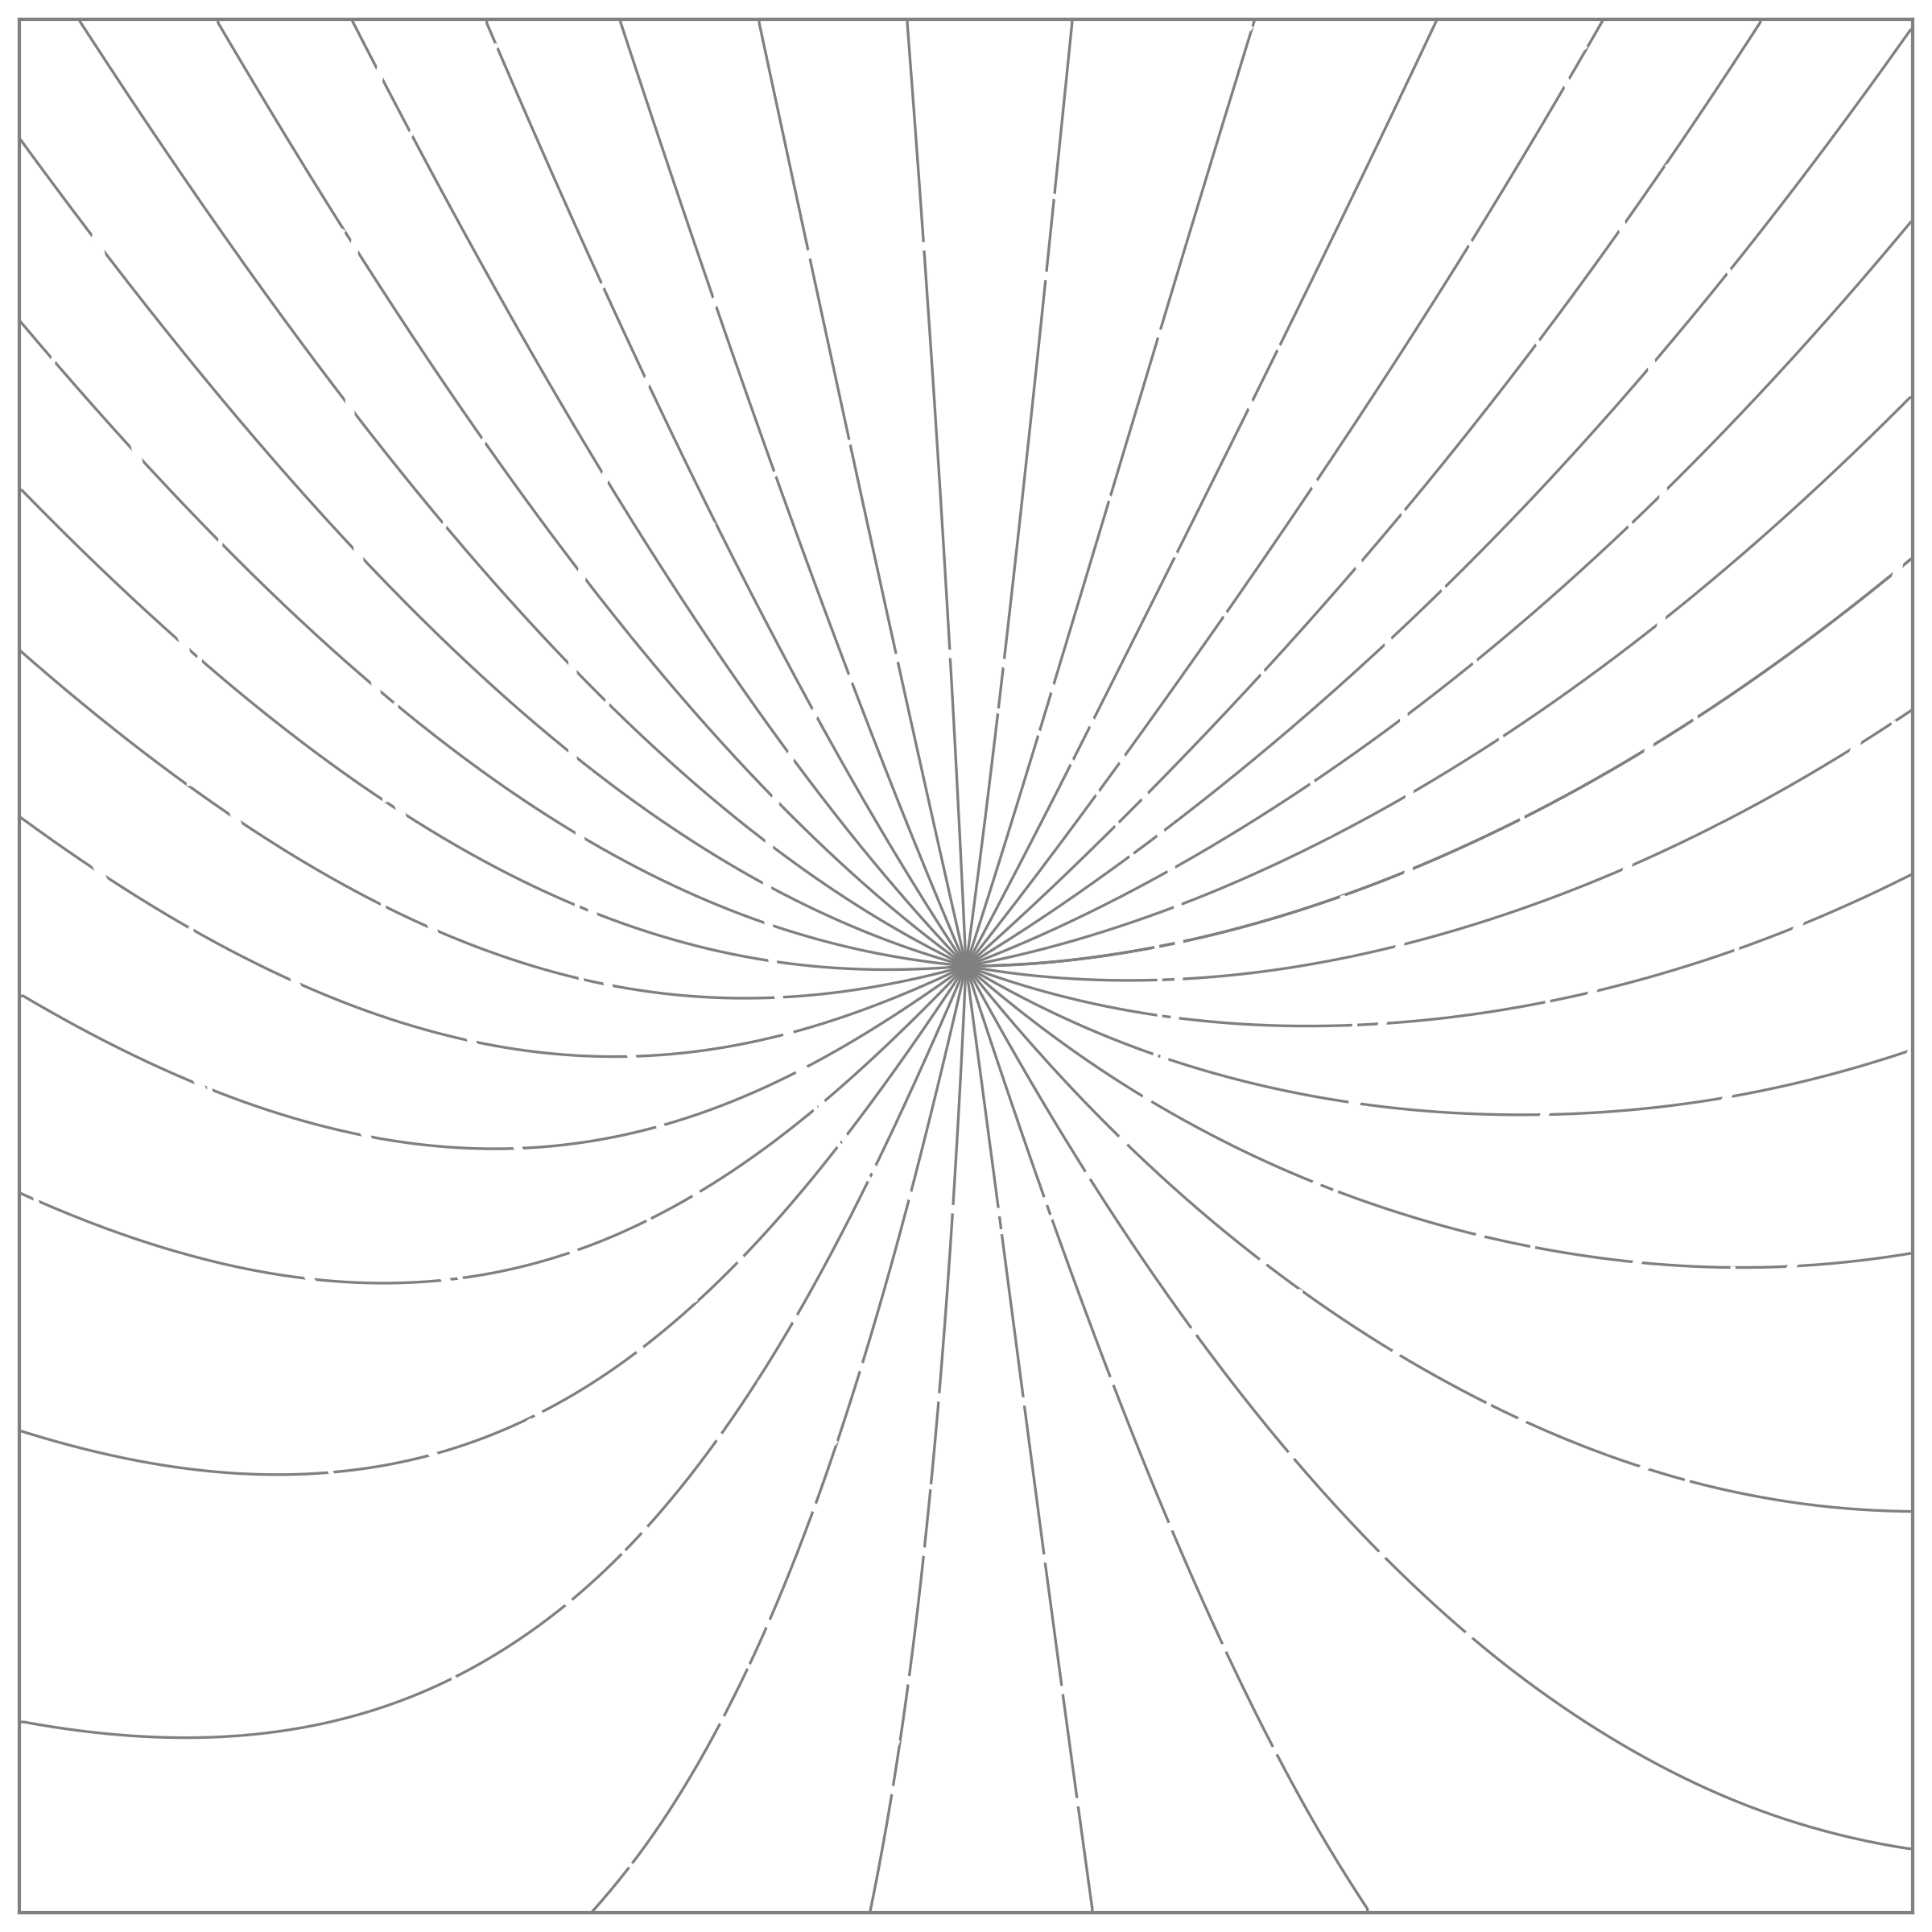
\includegraphics[width=0.6\textwidth]{cover_image.png}
    %\vspace*{2cm}

    \vfill

    \tpauthor{Dissertation\\[0.7cm]
    Johann Brehmer}

    \vspace*{2cm}

  \end{center}
\end{titlepage}



\end{document}
